\item

Problem 26.8-4

\begin{enumerate}
    \item 
    \begin{align*}
        \intertext{Species material balance around B and C}
        D_B &= 23.75 \text{ mol/h} \\
        D_C &= 1 \text{ mol/h} \\  
        W_B &= 1.25 \text{ mol/h} \\   
        W_C &= 19 \text{ mol/h} \\
        \intertext{Assume that there is no D in the distillate and no A in the worm}
        \Aboxed{D &=  64.75 \text{ mol/h}} \\
        \Aboxed{W &=  35.25 \text{ mol/h}}
    \end{align*}

    \item 
    \begin{align*}
        \intertext{Antoine's Equation}
        \ln P_{sat}^* = A - \frac{B}{T + C}    
    \end{align*}

    Antoine paramters:
    \begin{center}
        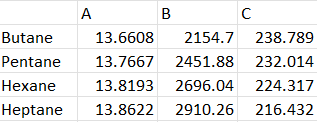
\includegraphics[width=0.5\textwidth]{assets/antoine.png}
    \end{center}

    \begin{align*}
        \intertext{In the distillate:}
        \intertext{Calculate vapor pressure for each species, guess temperature}
        K_i &= \frac{x_i}{P} \\
        \intertext{C is heavy key}
        \alpha_i &= \frac{K_i}{K_C} \\
        P &= \sum \frac{x_i}{\alpha_i} \\
        \intertext{Solve for dew point temperature}
        \Aboxed{T_{D} &= 65.8 \text{ $^\circ$C}} \\
        \intertext{In the worm:}
        \intertext{Calculate $K_i$ and $\alpha_i$}
        P &= \sum x_i\alpha_i \\
        \intertext{Solve for bubble point temperature}
        \Aboxed{T_{W} &= 129.8 \text{ $^\circ$C}} 
    \end{align*}

    \item 
    \begin{align*}
        \alpha_{avg} = \sqrt{\alpha_D \alpha_W} \\
        \alpha_{B, avg} &= 2.45 \\
        N_m &= \frac{\log\left[\left(\frac{x_{LD}}{x_{HD}}\right)\left(\frac{x_{HW}}{x_{LW}}\right)\right]}{\log\left(\alpha_{B, avg}\right)} \\
        \Aboxed{N_m &= 6.57} \\
        \intertext{Find composition of A in the worm and D in the distillate}
        \frac{x_{iD}}{x_{iW}} &= \left(\alpha_{i,avg}\right)^{N_m} \frac{x_{HD}}{x_{HW}} \\
        \Aboxed{x_{AW} &= 1.25\cdot10^{-4}} \\
        \Aboxed{x_{DD} &= 4.2\cdot10^{-5}} \\
        \intertext{Correct overall composition for new trace compositions}
    \end{align*}

    \item 
    \begin{align*}
        1-q &= \sum \frac{\alpha_ix_{iF}}{\alpha_i-\theta} \\
        & q = 1 \\
        \theta &= 1.22 \\
        R_m + 1 &= \sum \frac{\alpha_ix_{iD}}{\alpha_i-\theta} \\
        R_m + 1 &= 1.42 \\
        \Aboxed{R_m &= 0.426}
    \end{align*}

    \item 
    \begin{align*}
        \intertext{Use figure 26.8-3}
        \text{y-axis} &= \frac{R}{R+1} \\
        \text{tie lines} &= \frac{R_m}{R_m+1} \\
        R &= 0.554 \\
        \text{y-axis} &= 0.35 \\
        \text{tie lines} &= 0.29 \\
        \text{x-axis} &= 0.42 \\
        \text{x-axis} &= \frac{N_m}{N} \\
        \Aboxed{N &= 15.6}
    \end{align*}
    
    \item 
    \begin{align*}
        \log \left(\frac{N_e}{N_s}\right) &= 0.206 \log\left[\left(\frac{x_{HF}}{x_{LF}}\right)\frac{W}{D}\left(\frac{x_{LW}}{x_{HD}}\right)^2\right] \\
        N_e + N_s &= 15.6 \\
        \intertext{Solve for $N_e$ and $N_s$}
        \Aboxed{N_e &= 8.5} \\
        \Aboxed{N_s &= 7.15}
    \end{align*}
\end{enumerate}